\documentclass[final]{siamltex}
%\usepackage{CJK}
%\usepackage{CJKnumb}
\usepackage{graphicx}
\usepackage{amsfonts}
\usepackage{amsmath}
\usepackage{amssymb}
\usepackage{fancyhdr}
\usepackage{indentfirst}
%\usepackage{titlesec}
\usepackage{placeins}
\usepackage{listings}
\usepackage{caption}
\usepackage{subfigure}
\usepackage{url}
\usepackage{bm}
\usepackage{dsfont}
\usepackage{comment}
\usepackage{titlesec}
\usepackage{multirow}
\usepackage{xcolor}
\usepackage{algorithm}
\usepackage{algpseudocode}
\renewcommand{\baselinestretch}{1.2}
\topmargin 0cm \oddsidemargin 0.66cm \evensidemargin 0.66cm
\textwidth 14.66cm \textheight 22.23cm
\parindent 5ex

\def\longrightharpoonup{\relbar\joinrel\rightharpoonup}
\def\longleftharpoondown{\leftharpoondown\joinrel\relbar}

\def\longrightleftharpoons{
  \mathop{
    \vcenter{
       \hbox{
       \ooalign{
          \raise1pt\hbox{$\longrightharpoonup\joinrel$}\crcr
  	  \lower1pt\hbox{$\longleftharpoondown\joinrel$}
	}
      }
    }
  }
}

\newcommand{\rates}[2]{\displaystyle \mathrel{\longrightleftharpoons^{#1\mathstrut}_{#2}}}
\newcommand{\cL}{{\mathcal L}}
\newcommand{\bR}{{\mathbb R}}
\newcommand{\argmin}{\mathop{\rm argmin}}%

\newcommand{\bE}{{\mathbf E}}

\newtheorem{remark}{Remark}
\titleformat{\subsubsection}[runin]{\normalfont\bfseries}{\thesubsection.}{3pt}{}

\begin{document}
\title{Applications of the cross-entropy method in diffusion processes}
%\author{Wei Zhang}
\author{Wei Zhang\textsuperscript{2}\and Han Wang\textsuperscript{1} \and
  Carsten Hartmann\textsuperscript{1,*}\and 
Marcus Weber\textsuperscript{2}\and Christof Sch\"{u}tte\textsuperscript{1,2}}
\footnotetext[1]{Institute of Mathematics, Freie Universit\"{a}t Berlin, Arnimallee 6, 14195 Berlin, Germany}
\footnotetext[2]{Zuse Institute Berlin, Takustrasse 7, 14195 Berlin, Germany}
\renewcommand{\thefootnote}{\fnsymbol{footnote}}
\footnotetext[1]{Corresponding author. Email: chartman@mi.fu-berlin.de}
\date{}
\maketitle
\begin{abstract}
  The cross-entropy method in the diffusion process setting is studied. The
  general algorithm is proposed and is applied to design efficient importance sampling for rare events as well as to solve optimal
  control problem of diffusion process. Several examples are studied
  numerically to demonstrate this method.
\end{abstract}
\begin{keywords}
importance sampling, optimal control, cross-entropy method, Monte Carlo
method, rare event, change of measure. 
\end{keywords}
\begin{AMS}
\end{AMS}
\section{Introduction}
\label{intro}
Diffusion process has been extensively investigated because of its wide
applications in mathematics, physics, economics, and so on.
Here we are mainly interested in two topics in diffusion process, i.e. importance sampling and optimal control. 
For importance sampling, it is one kind of variance reduction technique 
in Monte Carlo simulations and becomes especially necessary in rare event simulation.
For optimal control, the purpose is to driven the dynamical system in certain
optimal way and has strong applicational backgrounds in finance, climate
science, mechanics \cite{fleming2006}. We emphasize that these two different areas are actually related and can
be unified as the same problem, i.e. how to change the measure in certain optimal way.

Here we take an applied point of view, i.e. we aim at designing efficient
algorithms to find the way to do the importance sampling, or to find the
optimal control strategy. One main reason that designing efficient algorithms
is urgent and challenging is due to the high dimensionality of the dynamical
systems, as in the case of climate system, biological system and so on. However, when the dynamical
systems have multiscale feature, efficient algorithms may be designed by
taking this feature into account. See \cite{ip-dupuis-multiscale, ip-eric,
zhws13} on importance sampling and \cite{control_schuette, zlph2013} on
optimal control for more details.

In this work, we consider these two topics together as how to design the change of
measure in an optimal way. If we further assume the existence of the optimal
change of measure $\mu^*$, the problem can be roughly described as how to find the approximation of
$\mu^*$ under some measure distance. For the choice of measure distances, we will use the Kullback-Leibler
divergence, which, although not a metric, is
widely used to quantified the similarity of two probability measures. 
What is more, given certain target probability measure $\mu^*$, the so-called cross-entropy method has been
developed recently and provides a general algorithm to find the minimizer of the
Kullback-Leibler divergence w.r.t. $\mu^*$, among a family of parameterized
probability measures. It has wide applications in different areas, such as
Monte Carlo simulation, optimization, and machine learning \cite{ce_tutorial, ce_book}. The
main purpose of this paper is to formulate the cross-entropy method in the
context of diffusion process, i.e. for measures defined in path space, and
discuss the applications of this method in importance sampling and optimal control
problems.

This paper is organized as follows. In Section~\ref{sec-om-functional},
using Girsanov theorem, we derive the Onsager-Machlup functional for a given trajectory.
In Section~\ref{sec-ce-is}, the cross-entropy method in path space is
formulated for the importance sampling problem.
In Section~\ref{sec-ocp}, by using the dual relationship between importance
sampling and optimal control problem, we discuss the cross-entropy method for
optimal control problem. The cross-entropy algorithm is summarized in
Section~\ref{sec-ce-algo}. Several numerical examples are studied in
Section~\ref{sec-examples}. Discussions are presented in
Section~\ref{sec-discuss}.


\section{Onsager-Machlup functional}
\label{sec-om-functional}
Let $O \subset \mathbb{R}^n$, $z_s \in \mathbb{R}^n$ satisfies the SDE 
\begin{align}
\begin{split}
  d z_s &= b(z_s) ds + \sqrt{2\beta^{-1}} dw_s, \quad 0 < s < \tau  \\
  z_0&=x
  \end{split}
\label{dynamics-1}
\end{align}
$\beta >0$ is constant, $\tau = \inf_{s>0} \{s;\, z_s \in O\}$ is some
stopping time, $b : \mathbb{R}^n \rightarrow \mathbb{R}^n$, $w$ is a
$n$-dimensional Brownian motion. 

We derive the Onsager-Machlup functional for dynamics (\ref{dynamics-1}) in
this section.
Let $\mu$ and $\mu_0$ be the probability measures on path space generated by
(\ref{dynamics-1}) and the scaled Brownian motion
\begin{align}
  \begin{split}
  dz_s &= \sqrt{2\beta^{-1}}dw_s, \hspace{3mm} 0 < s < \tau \\
   z_0 &= x .
  \end{split}
\end{align}
From Girsanov theorem \cite{oksendalSDE}, we have 
\begin{align}
  \frac{d\mu}{d\mu_0} &= \exp\Big(\sqrt{\frac{\beta}{2}}\int_0^\tau
  \langle b(z_s), dw_s\rangle + \frac{\beta}{4}\int_0^\tau |b(z_s)|^2ds\Big) \notag\\
  &=\exp\Big(\frac{\beta}{2}\int_0^\tau \langle b(z_s),dz_s\rangle -
  \frac{\beta}{4}\int_0^\tau |b(z_s)|^2ds\Big) 
\end{align}
and
\begin{align}
  d\mu_0 = \exp\Big(-\frac{\beta}{4}\int_0^\tau
  \Big|\frac{dz}{ds}\Big|^2ds\Big) d\nu\,
\end{align}
where $\nu$ is the Wiener measure. Together we obtain
\begin{align}
  d\mu &=\exp\Big(-\frac{\beta}{2} I_{1}(z)\Big)d\nu
  \label{measure-1}
\end{align}
where
\begin{align}
  I_{1}(z) = \frac{1}{2}\int_0^\tau \Big|\frac{dz}{ds} - b(z_s)\Big|^2 ds
\end{align}
and the integral is interpreted as Ito integral.
We could also rewrite it as Stratonovich integral using the relationship
\begin{align}
  \int_0^\tau \langle b(z_s), dz_s\rangle = \int_0^\tau b(z_s) \circ dz_s - \beta^{-1} \int_0^\tau \operatorname{div}\,b(z_s) ds
\end{align}
and therefore obtain 
\begin{align}
  d\mu = \exp \Big(-\frac{\beta}{2} I_2(z) \Big) d\nu\,
\end{align}
where functional 
\begin{align}
  I_2(z) = \frac{1}{2}\int_0^\tau \Big|\frac{dz}{ds}- b(z_s)\Big|^2 ds +
  \beta^{-1} \int_0^\tau \operatorname{div}\,b(z_s) ds
  \label{om-fun}
\end{align}
is often called Onsager-Machlup functional \cite{om1978, om_functional_pinski}. 
\begin{remark}
  The introduction of Onsager-Machlup functional and Stratonovich integral is
  not necessary. However, it is helpful to allow us to follow the presentation of
  \cite{ce_tutorial}, \cite{ce_book} and to compare with the case of random
  variables.
\end{remark}
\begin{remark}
  \label{remark-general}
  The Onsager-Machlup functional can also be generalized to the following dynamics.
  \begin{enumerate}
    \item
      SDEs with non-constant diffusion coefficients. We consider 
      \begin{align}
	\vspace{-9mm}
    \begin{split}
      d z_s &= b(z_s) ds + \sqrt{2\beta^{-1}} \sigma(z_s)\,dw_s, \quad 0 < s < \tau \\
      z_0&=x
    \end{split}
    \label{dynamics-1-sigma}
    \end{align}
    where $a(z) = \sigma(z)\sigma(z)^T$ is $n \times n$ positive definite matrix. We have 
    $d\mu = \exp(-\frac{\beta}{2} I_1(z)) d\nu$, with 
    \begin{align*}
      I_1(z) = \frac{1}{2} \int_0^\tau \Big|\frac{dz}{ds} -
      b(z_s)\Big|_{a(z)}^2 ds
    \end{align*}
     where Ito integral is used and $|v|_a = \langle v, a^{-1}v\rangle$,
     $\forall v \in \mathbb{R}^n$.
    \item
      System contains both stochastic and deterministic equations. For
      simplicity, here we consider dynamics 
      \begin{align}
      \begin{split}
	dx_s & = b_1(x_s, y_s)\, ds \\
	dy_s & = b_2(x_s, y_s)\, ds + \sqrt{2\beta^{-1}} dw_s
      \end{split}
      \label{ode-sde}
      \end{align}
      where $x_s \in \mathbb{R}^k, y_s, w_s \in \mathbb{R}^{n-k}$, $b_1 :
      \mathbb{R}^k \times \mathbb{R}^{n-k} \rightarrow \mathbb{R}^k$, $b_2 :
      \mathbb{R}^k \times \mathbb{R}^{n-k} \rightarrow
      \mathbb{R}^{n-k}$. We can still assign a probability measure $\mu$ on the
      \textbf{trajectory space}, i.e. $\forall z = (x,y) $ is a trajectory, we have 
      $d\mu = \exp(-\frac{\beta}{2} I_1(z)) d\nu$, where $\nu$ is Wiener
      measure on $\mathbb{R}^{n-k}$ and 
      \begin{align*}
	I_1(z) = \frac{1}{2} \int_0^\tau \Big|\frac{dy}{ds} - b_2(x_s, y_s)
	\Big|^2 ds\,.
      \end{align*}
      Notice that only the stochastic equations are used.
  \end{enumerate}
\end{remark}
\section{Cross-entropy method for importance sampling}
\label{sec-ce-is}
In this section, we discuss how to apply the cross-entropy
method \cite{ce_tutorial, ce_book} to guide the
importance sampling in diffusion process.

Let $\mathcal{D}$ be certain subset in the path space and
$\textbf{1}_{\mathcal{D}}$ be the
characteristic function on $\mathcal{D}$. 
In the following, for simplicity, we will use $z$ to denote a path trajectory
$\{z_s\}$ and keep the notation $z_s \in \mathbb{R}^n$ for the state at time $s$. 
Let $F(\cdot)$ be certain path functional and will be written as $F(z)$ for
path $z$. 
We consider Monte Carlo method with importance sampling to compute the quantity
\begin{align}
  l = \mathrm{E}(F(z)~|~z_0 = x)
  \label{mean-l}
\end{align}
where we assume $F(\cdot)$ has the following type
\begin{align}
  F(z) = \textbf{1}_{\mathcal{D}}(z) \quad \mbox{or} \quad F(z) = \exp(-\beta\int_0^\tau G(z_s) \,ds).
  \label{path-fun-f}
\end{align}
  A special and interesting case is when $\mathcal{D} = \{z, \tau(z) \le \lambda\}$,
  $\lambda > 0$ is fixed. Then $l = \mathrm{E}(\textbf{1}_{\mathcal{D}}(z)) =
  \mathcal{P}(\tau \le \lambda)$, i.e. the probability of the trajectories
  stop before time $\lambda$. This quantity may provide us some details of the
  distribution of the stopping time $\tau$ and help us understand the
  behaviors of the dynamics.

We suppose $m$ basis functions on state space $\{\phi_i\}_{1\le i \le m}$ are
available, where $\phi_i : \mathbb{R}^n\rightarrow \mathbb{R}$. 
We will add a control force to the original dynamics (\ref{dynamics-1})
and the importance sampling will be realized by simulating trajectories from
this modified dynamics. Specifically, given $\bm{\omega} = (\omega_1, \omega_2,
\cdots, \omega_m)^T \in \mathbb{R}^m$,
the corresponding control force is state-dependent and is supposed to be 
\begin{align}
  u(x; \bm{\omega}) = \sum\limits_{i = 1}^{m} \omega_i \nabla \phi_i(x), \quad x \in
  \mathbb{R}^n\,.
  \label{control-force}
\end{align}
Therefore, for fixed parameter $\bm{\omega}$, the controlled dynamics is 
\begin{align}
\begin{split}
  d z_s &= b(z_s) ds + \sqrt{2}u(z_s;\bm{\omega}) ds + \sqrt{2\beta^{-1}} dw_s, \quad t \le s \le \tau \\
     z_0 &=z
  \end{split}
\label{dynamics-2}
\end{align}
Let $\mu_{\bm{\omega}}$ be the probability measure of dynamics (\ref{dynamics-2}). 
From Section \ref{sec-om-functional},  we know $\mu_{\bm{\omega}}$ has density 
$f(z;\bm{\omega}) = \exp(-\frac{\beta}{2} I(z ; \bm{\omega}))$ w.r.t. Wiener
measure $\nu$, with
\begin{align}
  I(z ; \bm{\omega}) = \frac{1}{2}\int_0^\tau \Big|\frac{dz}{ds}- b(z_s) -
  \sqrt{2}\sum\limits_{i = 1}^{m} \omega_i \nabla \phi_i(z_s)\Big|^2 ds + \beta^{-1}
  \int_0^\tau \operatorname{div}\, \Big(b(z_s) + \sqrt{2}\sum\limits_{i =
  1}^{m} \omega_i \nabla \phi_i(z_s)\Big) ds
  \label{om-fun-w}
\end{align}
and the original dynamics (\ref{dynamics-1}) corresponds to $\bm{\omega} = \bm{0}$ (we use $\mu = \mu_{\bm{0}}$).
Given a probability measure $\mu_g$ on path space with $d\mu_g = g(z)d\nu$, 
we can design a unbiased Monte Carlo estimator for (\ref{mean-l}) as 
\begin{align}
  l_N = \frac{1}{N} \sum_{i=1}^{N}  \frac{F(z_i)f(z_i;\bm{0})}{g(z_i)}
\end{align}
where trajectories $z_i, i = 1, \cdots, N$ are sampled from measure $\mu_g$.
The optimal measure $\mu_{g^*}$, which gives
zero-variance estimator, should satisfy 
\begin{align}
  g^*(z) = \frac{F(z)f(z;\bm{0})}{l}, \hspace{3mm} \forall z
  \label{optimal_pdf}
\end{align}
However, $g^*(z)$ depends on the path $z$ and is not easy to compute. 

The idea of cross-entropy method is to find the best approximation of $g^*(z)$ among
$f(z;\bm{\omega}), \bm{\omega} \in \mathbb{R}^m$. More specifically, define the
Kullback-Leibler divergence between
two measures $d\mu_1 = g_1d\nu$, $d\mu_2 = g_2d\nu$ as
\begin{align}
  D(\mu_1, \mu_2) = \mathrm{E}_{\mu_1} \log \frac{d\mu_1}{d\mu_2} = \int
  g_1\log g_1\, d\nu - \int g_1\log g_2\,d\nu,
  \label{kl-dist}
\end{align}
and we try to minimize
\begin{align}
  \min_{\bm{\omega} \in \mathbb{R}^m} D(\mu_{g^*}, \mu_{\bm{\omega}}).
  \label{kl-dist-d}
\end{align}
Using (\ref{optimal_pdf}) and (\ref{kl-dist}), it is equivalent to solve
\begin{align}
  \max_{\bm{\omega} \in \mathbb{R}^m} \mathrm{E}_{\mu} ( F(z) \log
  f(z;\bm{\omega}))
  = \max_{\bm{\omega} \in \mathbb{R}^m} \mathrm{E}_{\mu_{\bm{v}}} ( F(z)
  \eta(z;\bm{v}) \log f(z;\bm{\omega})), \hspace{3mm} \forall \bm{v} \in
  \mathbb{R}^m
  \label{ce-2}
\end{align}
where
\begin{align}
  \eta(z;\bm{v}) = \frac{f(z;\bm{0})}{f(z;\bm{v})}.
\end{align}
For numerical purpose, we consider the discrete formulation of (\ref{ce-2})
\begin{align}
\max_{\bm{\omega} \in \mathbb{R}^m} \frac{1}{N} \sum_{i=1}^{N} F(z_i)
\eta(z_i; \bm{v}) \log f(z_i;\bm{\omega}) 
\label{ce-2-discrete}
\end{align}
where $z_i, i = 1, \cdots, N$ are trajectories generated from $\mu_{\bm{v}}$. 
Taking gradient, the maximizer of (\ref{ce-2-discrete}) could be found by solving
\begin{align}
  \frac{1}{N} \sum_{i=1}^{N} F(z_i) \eta(z_i; \bm{v}) \nabla_{\bm{\omega}} \log
  f(z_i;\bm{\omega}) = 0.
  \label{max-gradient}
\end{align}
With formula (\ref{om-fun-w}), equations (\ref{max-gradient}) could be written more explicitly
as linear equations $A\bm{\omega} = \bm{r}$, where $\forall 1\le i,j\le m$, 
\begin{align}
  \begin{split}
  A_{ij} &= \frac{1}{N}\sum_{k = 1}^{N} F(z_k)\eta(z_k; \bm{v}) \int_0^\tau
  \nabla\phi_i(z_{k,s})\nabla\phi_j(z_{k,s})\,ds, \\
     r_i &= \frac{1}{\sqrt{2}N}\sum_{k = 1}^{N} F(z_k)\eta(z_k; \bm{v})
  \Big[\int_0^\tau \Big(\frac{dz_k}{ds} - b(z_s)\Big)\nabla\phi_i(z_{k,s})\,ds
  - \beta^{-1} \int_0^\tau \operatorname{div} \nabla \phi_i(z_{k,s})\,ds\Big]
  \end{split}
  \label{linear-eqn}
\end{align}
Notice that (\ref{max-gradient}) holds $\forall \bm{v} \in \mathbb{R}^m$ and
$A$ is in general a positive definite matrix when $\phi_i$'s are linearly independent.
\begin{remark}
  The more general type conditional expectation 
  $l = \mathrm{E}(F(z)~|~ z_0 \sim \pi)$
  can be similarly considered,
where $\pi(dx) = \rho(x)dx$ is a probability measure on $\Omega
\subset \mathbb{R}^n$, i.e. $\int_\Omega \rho(x)\,dx = 1$. Let $E = \{z ~|~ z \in
  C([0,\infty), \mathbb{R}^n), z_0 \in \Omega\}$ be the set of trajectories
  starting from $\Omega$. Denote $\mu^x$ as the aforementioned measure for
  dynamics (\ref{dynamics-1}) starting from $x \in \mathbb{R}^n$. Further
  define $\mu^\pi(\mathcal{D}) = \int_{\Omega} \mu^x(\mathcal{D}) \pi(dx)$,
  where $\mathcal{D}$ is a measurable subset of $E$.
  We have $d\mu^\pi_{\bm{v}} = f(z;\bm{v})\,d\nu^\pi, \forall
  \bm{v} \in \mathbb{R}^n$, where $\mu^\pi_{\bm{v}}$ and $\nu^{\pi}$ are
  defined similarly. The aim is to find the optimal $\bm{\omega} \in
  \mathbb{R}^m$ and the corresponding measure $\mu^\pi_{\bm{\omega}}$ to do
  the importance sampling. All the derivations are the same with the above
  except that, while simulating the trajectories, 
  the starting point $z_0$ should be generated from $z_0 \sim \pi$.
\end{remark}
\begin{remark}
   The above algorithm can be further applied to dynamics (\ref{ode-sde}), discussed
   in Remark \ref{remark-general}. In this case, since only stochastic
   equations appear in the Radon-Nikodym derivative, the control should
   also be only added to these equations, in order to obtain linear equations
   with full rank. Specifically, we study the controlled dynamics 
         \begin{align}
      \begin{split}
	dx_s & = b_1(x_s, y_s)\, ds \\
	dy_s & = b_2(x_s, y_s)\, ds + \sqrt{2} u(x_s, y_s ; \bm{\omega})\, ds + \sqrt{2\beta^{-1}} dw_s
      \end{split}
      \label{ode-sde-control}
      \end{align}
      with $u(x_s, y_s ; \bm{\omega}) = \sum\limits_{i=1}^{m} \omega_i \nabla \phi_i(x_s,
      y_s)$ and optimize the coefficients $\bm{\omega}$. All the derivations are
      the same as above.
\end{remark}
\section{Cross-entropy method for optimal control problem}
\label{sec-ocp}
In this section, we consider applying the cross-entropy method to solve optimal control problem
for diffusion process.

Consider the optimal control problem with cost
function \cite{control_schuette,zlph2013}
\begin{equation}
  J(u) = \mathrm{E}_{\mu_u}\left[\int_0^\tau \left(G(z_s) + \frac{1}{2} |u(z_s,s)|^2
\right) ds ~\bigg|~ z_0 = x\right],
\end{equation}
where $G : \mathbb{R}^n\rightarrow \mathbb{R}$ is nonnegative, $u$ is the
control force and $\mathrm{E}_{\mu_u}$ denotes the expectation under probability measure $\mu_u$,
which is generated by the controlled dynamics
of (\ref{dynamics-1-sigma}), namely,
\begin{align}
 \begin{split}
   d z_s &= b(z_s) ds + \sqrt{2}\sigma(z_s) u(z_s, s) ds + \sqrt{2\beta^{-1}} \sigma(z_s)\,dw_s, \quad 0 < s < \tau \\
    z_0&=x
  \end{split}
  \label{dynamics-1-sigmma-c}
\end{align}

Suppose the lower bound of $J(u)$ can be achieved and let $\hat{u} = \argmin J(u)$. For simplicity, we denote $\mu, \hat{\mu}$ as
the probability measure corresponding to $u \equiv 0$ and $\hat{u}$
respectively. Using the dual relation \cite{DaiPra1996, zlph2013}
    \begin{align}
      -\beta^{-1}\log \mathrm{E}_\mu\left[\exp\Big(-\beta\int_0^\tau G(z_s)\, ds\Big)\right] = \inf_u J(u) = J(\hat{u})
      \label{dual-relation}
    \end{align}
    and Jensen's inequality, we know that 
    \begin{align}
    \exp\Big(-\beta\int_0^\tau G(z_s)\,ds\Big)\frac{d\mu}{d\hat{\mu}} =
    \mathrm{E}_\mu\left[\exp\Big(-\beta\int_0^\tau G(z_s)\, ds\Big)\right],
    \hspace{3mm} \hat{\mu}-a.s.
    \label{jensen-as}
  \end{align}
From the above we have 
  \begin{align}
    J(u) &= \mathrm{E}_{\hat{\mu}} \left\{\Big[\int_0^\tau \Big(G(z_s) + \frac{1}{2} |u(z_s,
    s)|^2\Big)\,ds\Big]\frac{d\mu_u}{d\hat{\mu}}\right\}  \\
    & = J(\hat{u}) + \mathrm{E}_{\hat{\mu}}\Big[\Big(\beta^{-1}\log
    \frac{d\mu}{d\hat{\mu}} + \int_0^\tau \frac{1}{2} |u(z_s,
    s)|^2\,ds\Big)\frac{d\mu_u}{d\hat{\mu}}\Big]
\end{align}
After simplification, we get the following simple relationship 
\begin{align}
J(u) = J(\hat{u}) + \beta^{-1}D(\mu_u|\, \hat{\mu}).
\label{J-entropy}
\end{align}
where $D(\cdot, \cdot)$ is the Kullback-Leibler divergence in (\ref{kl-dist}).

We are interested in finding the optimal control $\hat{u}$. For high
dimensional dynamics ($n$ is large), this becomes difficult.  
Similarly as the in previous section, we suppose the control force can be written
as (\ref{control-force}) with $m$ predefined basis functions $\{\phi_i\}_{1\le
i \le m}$. And our problem is simplified to solve
\begin{align}
  \min_{\bm{\omega} \in \mathbb{R}^m} J(u(z;\bm{\omega})).
  \label{J-w}
\end{align}
under dynamics (\ref{dynamics-1-sigmma-c}).

From (\ref{J-entropy}), we know that solving (\ref{J-w})
is equivalent to minimize the Kullback-Leibler divergence $D$ between
$\mu_u$ and $\hat{\mu}$, which, however, is still not easy. On the other hand, inspired by 
the discussions in Section \ref{sec-ce-is}, we can apply cross-entropy method 
to minimize $D(\hat{\mu} \,|\, \mu_u)$ (notice this is different from
(\ref{J-w}), because the Kullback-Leibler divergence is not symmetric), and
hope that (\ref{J-w}) can be solved approximately. Following
the notations in Section \ref{sec-ce-is} and from (\ref{jensen-as}), we know the optimal measure
satisfies
\begin{align}
  g^*(z) \propto \exp\Big(-\beta\int_0^\tau G(z_s) \,ds\Big) f(z ; 0),
  \quad \forall z\,,
\end{align}
therefore the problem is reduced to the case in Section \ref{sec-ce-is} with $F(z) = \exp(-\beta\int_0^\tau G(z_s) \,ds)$.
\section{Cross-entropy algorithm}
\label{sec-ce-algo}
In this section, we consider how to implement the cross-entropy algorithm in
order to maximize (\ref{ce-2-discrete}), which is equivalent to (\ref{kl-dist-d}) in the discrete case. 
We suppose the optimal density $g^*(z)$ is given by (\ref{optimal_pdf}) and
$F(z)$ takes the forms in (\ref{path-fun-f}).

Ideally, the solution of the maximization problem (\ref{ce-2-discrete}) can be
obtained by solving the linear equation (\ref{linear-eqn}) without iterations. But in real
applications, when the expectation value $l$ of $F(z)$ in (\ref{mean-l}) is very rare, it will become
difficult to estimate the coefficients (\ref{linear-eqn}) and therefore the solution
will be inaccurate. In diffusion processes, one major reason for this rarity
is the metastability in the dynamics when $\beta \gg 1$. In this case, the
trajectories are long and $F(z)$ is small, which means computing
(\ref{linear-eqn}) is both time-consuming and inaccurate. Inspired by the
original cross-entropy method \cite{ce_tutorial},
we may overcome this problem by starting from a higher temperature (smaller $\beta$) and compute
(\ref{linear-eqn}) while decreasing the temperature (increasing $\beta$). The proposed iterative
method to solve the maximization problem (\ref{ce-2-discrete}) is illustrated in Algorithm \ref{ce-algo}.
\begin{algorithm}
  \caption{Algorithm to solve the maximization problem (\ref{ce-2-discrete}) \label{ce-algo}}
  \begin{algorithmic}[1]
    \State Define $0 < \beta_0 < \beta_1 < \cdots <\beta_k = \beta$, set
    $\bm{v}^{(0)} = 0$.
    \For {$j=0$ to $k$}
    \State generate $N_j$ trajectories $z_i, i=1,2,\cdots, N$ from dynamics (\ref{dynamics-2}), with
    $\bm{\omega} = \bm{v}^{(j)}$, $\beta = \beta_j$.
    \State compute the coefficients of $A^{(j)}, \bm{r}^{(j)}$ from (\ref{linear-eqn}) with $\bm{v} =
    \bm{v}^{(j)}$, and solve the linear equations $A^{(j)}\bm{v}^{(j+1)} =
    \bm{r}^{(j)}$.
    \EndFor 
  \end{algorithmic}
  \label{algo1}
\end{algorithm}
\FloatBarrier
\section{Numerical examples}
\label{sec-examples}
In this section, we will study the cross-entropy method with some concrete dynamics and
illustrate some numerical results.
\subsection{One-dimensional double well potential}
Here we consider the simplest 1D diffusion process with double well potential.
Let $b(x) = - V'(x), x\in \mathbb{R}^1$, with $V(x) = \frac{1}{2}(x^2 - 1)^2$.
The dynamics is 
\begin{align}
  dz_s = - V'(z_s) ds + \sqrt{2\beta^{-1}} dw_s
\end{align}
where $w_s$ is 1D Brownian motion. The potential $V$ has two minima points
$x_0 = -1, x_2 = 1$, while $x_1 = 0$ is
a saddle point. Define $\tau = \inf\{s >0, |z_s - x_2| \le 1 \}$, and choose
the starting point $z_0 = x_0 =
-1$. We define three basis functions of Gaussian type as $\phi_i(x) = \exp(-\frac{(x -
x_i)^2}{2r^2})$, $i = 0, 1, 2$, and choose $r = 0.5, \beta = 5.0$ (see Figure. \ref{fig-ex1-basis}).

We first study the optimal control problem  
\begin{align}
  \inf_{u_s} \mathrm{E} \Big(\tau + \frac{1}{2} \int_0^\tau u_s^2 \,ds~\Big|~
  z_0 = -1\Big)\,,
  \label{ex1-cost}
\end{align}
under dynamics
\begin{align}
  dz_s = - V'(z_s) ds + \sqrt{2}u_s ds + \sqrt{2\beta^{-1}} dw_s\,.
\end{align}
$\mbox{dt} = 1.0 \times 10^{-3}$, $N_j = 10^{4}, j=0,1,2$ are used to compute the
coefficients $\bm{\omega}$ using Algorithm.\ref{ce-algo}, with $\{\beta_0,\beta_1, \beta_2\}
= \{1.0, 3.0, 5.0\}$.  Therefore $k=2$ in Algorithm.\ref{ce-algo} and $3$
iteration steps are performed. Denote $\bm{v}^{(0)} = \bm{0}$ and suppose
coefficients $\bm{v}^{(j+1)}$ are obtained
in $j$th steps, $j=0,1,2$. Then applying control force $u(x;\bm{v}^{(j)})$ is
equivalent to modifying the potential as $V^{(j)}(x) = V(x) - \sqrt{2}\sum\limits_{i=0}^{2} v^{(j)}_i
\phi_i(x)$. The numerical results are presented in Figure.\ref{fig-ex1-1} and Figure.\ref{fig-ex1-2}.
In Figure.\ref{fig-ex1-1}, we show the modified potential $V^{(j)}(x), 0\le
j\le 3$ when different basis functions are used. We can observe that the potential is
gradually modified during the iterations. In Figure.\ref{fig-ex1-2}, it shows
the modified potentials $V^{(3)}(x)$ with optimized coefficients
$\bm{v}^{(3)}$ in Algorithm.\ref{ce-algo} for different basis functions. In
one-dimension, the optimal control problem (\ref{ex1-cost}) can also be solved
from a Feymann-Kac type boundary value PDE \cite{control_schuette}. The
potential (the cost value) obtained in this way can be considered as the exact solution and is also
shown in Figure.\ref{fig-ex1-2} (The last row of Tab.~\ref{tab-ex1-1}).
Later on, $N = 10^{6}$ samples are generated to compute
the cost function (\ref{ex1-cost}) and the results are presented in
Tab.~\ref{tab-ex1-1}. We can observe that better results are obtained when basis function
$\phi_1$ is used, since in job 2 and 3, the cost value (1.31) is closer to the exact
solution (1.25). Notice that this fact is also shown in
Figure.\ref{fig-ex1-2}, as the potential profiles with Label ``basis 0, 1'' and
Label ``basis 1'' are more similar to the profile with Label ``exact'', the
optimal potential. (Notice that only the region $x<0$ is meaningful and the dynamics remains the same when
the potential is shifted vertically) 
\begin{figure}[tphb]
  \centering
\includegraphics[width=7cm]{./fig/basis_1d.eps}
\caption{One-dimensional basis functions $\phi_0, \phi_1, \phi_2$. \label{fig-ex1-basis}}
\end{figure}
\begin{figure}[tphb]
  \centering
  \begin{tabular}{ll}
    \subfigure[basis $\phi_0$]{\includegraphics[width=5.0cm]{./fig/pot_1d_0_converge_control.eps}}
&
    \subfigure[basis $\phi_1$]{\includegraphics[width=5.0cm]{./fig/pot_1d_1_converge_control.eps}} \\
    \subfigure[basis $\phi_0,\phi_1$]{\includegraphics[width=5.0cm]{./fig/pot_1d_2_converge_control.eps}}
    &
    \subfigure[basis $\phi_0,\phi_2$]{\includegraphics[width=5.0cm]{./fig/pot_1d_3_converge_control.eps}}
\end{tabular}
\caption{Optimal control problem for one-dimensional dynamics. Convergence results for the modified
potentials $V^{(j)}, j=0,1,2,3$, with different sets of basis functions\label{fig-ex1-1}}
\end{figure}
\begin{figure}[tphb]
  \centering
    \includegraphics[width=7.0cm]{./fig/pot_1d_basis_control.eps}
    \caption{Optimal control problem for one-dimensional dynamics. Optimized potential $V^{(3)}$ with
    different sets of basis functions. The curve with Label ``exact'' is
  computed directly by solving a Feymann-Kac boundary value PDE. \label{fig-ex1-2}}
\end{figure}
\begin{table}
  \centering
%  \begin{tabular}{c|c|c|c|c}
  \begin{tabular*}{0.8\textwidth}{@{\extracolsep{\fill}}ccccc}
    \hline
    \hline
    job & coefficients & cost & relative variance & mean of $\tau$ \\
    \hline
       $1$ & $(-1.771, 0, 0)$ & $5.14$ & $1.35$ & $2.02$  \\
       $2$ & $(0, 1.857, 0)$ & $1.31$ & $0.44$ & $0.57$  \\
       $3$ & $(-0.110, 1.762, 0)$ & $1.31$ & $0.44$ & $0.57$  \\
       $4$ & $(-1.611, 0, 1.379)$ & $3.88$ & $1.22$ & $1.73$  \\
       $5$ & $$ & $1.25$ & $0.30$ & $0.52$  \\
    \hline
    \hline
  \end{tabular*}
  \caption{Results of the optimal control problem for the one-dimensional dynamics with different sets
  of basis functions. The coefficients are solved by Algorithm.\ref{ce-algo}.
Job $1$-$4$ are the results with different sets of functions $\{\phi_0\}$,
$\{\phi_1\}$, $\{\phi_0, \phi_1\}$, $\{\phi_0, \phi_2\}$ respectively. The
costs are the exectation (\ref{ex1-cost}) computed with $N=10^6$ samples. The
last column is the mean of the stopping time $\tau$ under the modified
dynamics. The last row is the computed by solving a Feymann-Kac type PDE and
is considered as the ``accurate'' solution.\label{tab-ex1-1}}
\end{table}

We continue to study the computation of $P(\tau \le \lambda)$ for $\lambda > 0$.
We choose $\lambda = 2.0, 1.0, 0.5, 0.3, 0.1$ and two sets of basis functions are used : $\{\phi_1\}$
and $\{\phi_2\}$. We compare the results using importance sampling with the
standard Monte Carlo method. These results are shown in
Tab.~\ref{tab-ex1-2}--\ref{tab-ex1-4} and Figure.\ref{fig-ex1-3}.
Tab.~\ref{tab-ex1-2} and Tab.~\ref{tab-ex1-3} shows the results of
importance sampling with basis function $\{\phi_0\}$ and $\{\phi_1\}$,
respectively, while Tab.~\ref{tab-ex1-4} is the result using standard Monte Carlo method.
In each case, we can observe that the estimators' relative variance will increase when $\lambda$ becomes
small. However, for fixed $\lambda$, the relative variances of importance
sampling are largely reduced comparing to the standard Monte Carlo method. And this becomes
more apparent when $\lambda$ decreases, while the standard Monte Carlo method
may fail to work (see the last row of Tab.~\ref{tab-ex1-4}).
In Figure.\ref{fig-ex1-3}, the optimized potentials used to perform importance sampling
are ploted for different $\lambda$ and different sets of basis functions. As
$\lambda$ decreases,
the optimized potentials become more different from the original
potential, which indicates larger forces are needed.

\begin{table}
\centering
  \begin{tabular*}{0.9\textwidth}{@{\extracolsep{\fill}}cccccc}
    \hline
    \hline
   $\lambda$ & coefficients & $P(\tau \le \lambda)$ & relative variance & Traj. Usage & time (sec.) \\
    \hline
  $2.0$ & $(-0.837, 0, 0)$ & $9.22 \times 10^{-2}$ & $1.45$ & $6.1 \times 10^{-1}$ & $70.4$ \\
    $1.0$ & $(-1.391, 0, 0)$ & $3.23 \times 10^{-2}$ & $1.48$ & $4.8 \times 10^{-1}$ & $39.4$ \\
    $0.5$ & $(-2.221, 0, 0)$ & $6.45 \times 10^{-3}$ & $1.75$ & $3.9 \times 10^{-1}$ & $21.5$ \\
    $0.3$ & $(-3.282, 0, 0)$ & $9.51 \times 10^{-4}$ & $2.30$ & $3.3 \times 10^{-1}$ & $13.6$ \\
    $0.2$ & $(-4.553, 0, 0)$ & $9.53 \times 10^{-5}$ & $3.10$ & $2.7 \times 10^{-1}$ & $9.4$ \\
    $0.1$ & $(-8.245, 0, 0)$ & $1.22 \times 10^{-7}$ & $6.84$ & $1.6 \times
 10^{-1}$ & $4.9$ \\
    \hline
    \hline
  \end{tabular*}
  \caption{ $\mathcal{P}(\tau \le \lambda)$ for one-dimensional dynamics.
  $N=10^6$ samples and importance sampling are used with basis function
  $\{\phi_0\}$. ``Traj. Usage'' is the
ratio of trajectories satisfying $\tau \le \lambda$ under the modified dynamics. \label{tab-ex1-2}}
\end{table}
\begin{table}
  \centering
  \begin{tabular*}{0.9\textwidth}{@{\extracolsep{\fill}}cccccc}
    \hline
    \hline
    $\lambda$ & coefficients & $P(\tau \le b)$ & relative variance & Traj. Usage & time (sec.) \\
    \hline
  $2.0$ & $(0, 0.962, 0)$ & $9.23 \times 10^{-2}$ & $1.04$ & $8.5 \times 10^{-1}$ & $56.1$\\
  $1.0$ & $(0, 1.498, 0)$ & $3.23 \times 10^{-2}$ & $1.00$ & $8.1 \times 10^{-1}$ & $32.7$ \\
  $0.5$ & $(0, 2.314, 0)$ & $6.46 \times 10^{-3}$ & $1.33$ & $6.8 \times 10^{-1}$ & $19.4$ \\
  $0.3$ & $(0, 3.338, 0)$ & $9.49 \times 10^{-4}$ & $1.84$ & $5.6 \times 10^{-1}$ & $12.8$ \\
  $0.2$ & $(0, 4.578, 0)$ & $9.56 \times 10^{-5}$ & $2.54$ & $4.6 \times 10^{-1}$ & $9.02$\\
  $0.1$ & $(0, 8.232, 0)$ & $1.21 \times 10^{-7}$ & $5.28$ & $2.6 \times 10^{-1}$ & $4.8$\\
    \hline
    \hline
  \end{tabular*}
  \caption{ $\mathcal{P}(\tau \le \lambda)$ for one-dimensional dynamics.
  $N=10^6$ samples and importance sampling are used with basis function
$\{\phi_1\}$. ``Traj. Usage'' is the ratio of trajectories satisfying $\tau \le \lambda$ under the modified dynamics. \label{tab-ex1-3}}
\end{table}
\begin{table}
  \centering
  \begin{tabular*}{0.9\textwidth}{@{\extracolsep{\fill}}ccccc}
    \hline
    \hline
    $\lambda$ & $P(\tau \le \lambda)$ & relative variance & Traj. Usage & time (sec.) \\
    \hline
    $2.0$ & $9.23 \times 10^{-2}$ & $3.14$ & $9.23 \times 10^{-2}$ & $95.0$ \\
    $1.0$ & $3.22 \times 10^{-2}$ & $5.48$ & $3.22 \times 10^{-2}$ & $48.8$ \\
    $0.5$ & $6.28 \times 10^{-3}$ & $12.58$ & $6.28 \times 10^{-3}$ & $24.6$ \\
    $0.3$ & $1.00 \times 10^{-3}$ & $31.61$ & $1.00 \times 10^{-3}$ & $14.9$ \\
    $0.2$ & $9.30 \times 10^{-5}$ & $103.69$ & $9.30 \times 10^{-5}$ & $9.9$ \\
    $0.1$ & $0.00$ & $-$ & $0.00$ & $5.0$ \\
    \hline
    \hline
  \end{tabular*}
  \centering
  \caption{$\mathcal{P}(\tau \le \lambda)$ for one-dimensional dynamics.
    ``Traj. Usage'' is the
ratio of trajectories satisfying $\tau \le \lambda$ . $N=10^6$ samples are
used with standard Monte Carlo method. In the last row, the estimation fails because there is no
  trajectories satisfying $\tau \le \lambda$ among $N=10^6$ trajectory samples. \label{fig-ex1-3}}
\end{table}
\begin{figure}[tphb]
  \centering
  \begin{tabular}{lll}
    \subfigure[basis $\phi_0$]{\includegraphics[width=5.0cm]{./fig/pot_1d_1_b_ip.eps}}
    &
    \subfigure[basis $\phi_1$]{\includegraphics[width=5.0cm]{./fig/pot_1d_2_b_ip.eps}}
    &
    \subfigure[$P(\tau \le \lambda)$]{\includegraphics[width=5.0cm]{./fig/pdf_tau.eps}}
\end{tabular}
\caption{The modified potentials for computing $\mathcal{P}(\tau \le \lambda)$ of
one-dimensional dynamics with different sets of basis functions. The
potentials
become more different from the original one when $\lambda$ decreases. (c) shows the cumulative distribution function of
$\tau$ (only for small $\lambda$). \label{tab-ex1-4}} 
\end{figure}
%\FloatBarrier
%\subsection{Non-gradient dynamical system}
%Possibly more interesting examples are the noise-driven non-gradient
%systems studied in \cite{mechanism_coherence, stochastic_resonance}.
\subsection{Two dimensional example}
We choose the potential 
\begin{align}
V(x) = (1 - x_1^2 - x_2^2)^2 + \frac{x_1^2}{x_1^2 + x_2^2}, \quad x = (x_1,x_2) \in \mathbb{R}^2
\end{align}
and consider the two-dimensional dynamics
\begin{align}
  dz_s = - \nabla V(z_s) ds + \sqrt{2\beta^{-1}} dw_s
\end{align}
where $w_s$ is a two-dimensional Brownian motion.
The potential $V(x)$ (see Figure.\ref{fig-ex2-0}) has two minima at $a = (-1, 0)$ and $b = (1,0)$.
$c_1 = (0, 1)$ and $c_2 = (0,-1)$ are two saddle points and $d=(0,0)$ is a
singular point. The basis functions we choose are 
\begin{align}
  & \phi_0(x) = \exp(-\frac{|x - a|^2}{2r_0^2}), \quad \phi_1(x) = \exp(-\frac{|x - c_1|^2}{2r_1^2}), \\
  & \phi_2(x) = \exp(-\frac{|x - c_2|^2}{2r_2^2}) \quad \phi_3(x) = \exp(-\frac{|x|^2}{2r_0^2}) 
\end{align}
with $r_0 = 0.5, r_1 = r_2 = 1.0$. We study the dynamics starting from $z_0 =
a$ and define the stopping time as $\tau = \inf\{s > 0, |z_s - b| \le 1.0\}$.

For the optimal control problem, we consider the cost function 
\begin{align}
  \inf_{u_s} \mathrm{E}\Big(\tau + \frac{1}{2}\int_0^\tau |u_s|^2 ds ~\Big|~ z_0 = a \Big)
  \label{cost-ex2}
\end{align}
under dynamics
\begin{align}
  dz_s = - \nabla V(z_s) ds + \sqrt{2}u_s ds + \sqrt{2\beta^{-1}} dw_s
\end{align}
We choose $\beta = 8.0$, $\mbox{dt} = 0.001$. When solving the coefficients
using Algorithm.\ref{ce-algo}, we
choose $(\beta_0, \beta_1 , \beta_2, \beta_3) = (2.0, 4.0, 6.0, 8.0)$, and
$N_i = 10^4$ for each $\beta_i, i = 0, 1, 2, 3$. Four different sets of
basis functions $\{\phi_0\}$, $\{\phi_0, \phi_1\}$, $\{\phi_0, \phi_1,
\phi_2\}$, $\{\phi_0, \phi_1, \phi_2, \phi_3\}$ are studied. After finding the coefficients, the cost function (\ref{cost-ex2}) is computed with $N =
10^6$ samples. Results are tabulated in Tab.~\ref{tab-ex2-1}. From the dual relation
(\ref{dual-relation}), we also compute the optimal cost by Monte Carlo method
and the value is $1.27$. It can be observed that the cost ($1.39$) is close to the
optimal cost ($1.27$) if all basis functions are used. Figure.\ref{fig-ex2-1} shows the optimized potential with different basis functions.
\begin{figure}[tphb]
  \centering
    \includegraphics[width=7.5cm]{./fig/pot_2d_1_0_0.eps}
    \caption{Potential $V(x)$ for the 2D example. \label{fig-ex2-0}}
\end{figure}
\begin{table}[tphb]
  \begin{tabular*}{0.9\textwidth}{@{\extracolsep{\fill}}ccccc}
    \hline
    \hline
    job & coefficients & cost & relative variance & mean of $\tau$ \\
    \hline
    $0$ & ($-1.535$, $0.000$, $0.000$, $0.000$) & $3.69$ & $0.67$ & $2.97$ \\
    $1$ & ($-1.379$, $0.744$, $0.000$, $0.000$) & $3.86$ & $0.82$ & $3.16$ \\
    $2$ & ($-0.943$, $1.527$, $1.500$, $0.000$) & $2.48$ & $0.94$ & $1.71$ \\
    $3$ & ($-0.909$, $0.479$, $0.484$, $0.936$) & $1.39$ & $0.46$ & $0.63$ \\
    \hline
    \hline
  \end{tabular*}
  \centering
  \caption{2D example, optimal control problem with different sets of basis
  functions $\{\phi_0\}$, $\{\phi_0, \phi_1\}$, $\{\phi_0, \phi_1, \phi_2\}$, $\{\phi_0, \phi_1, \phi_2, \phi_3\}$.
  The coefficients are solved using Algorithm.\ref{ce-algo}. The cost value is
  computed with $N=10^{6}$ trajectories.
The last column is the mean value of stopping time $\tau$ under the modified
dynamics. \label{tab-ex2-1}}
\end{table}
\begin{figure}[tphb]
  \centering
  \begin{tabular}{ll}
    \subfigure[basis $\{\phi_0\}$]{\includegraphics[width=6.0cm]{./fig/pot_2d_1_0_4.eps}} 
    &
    \subfigure[basis $\{\phi_0, \phi_1\}$]{\includegraphics[width=6.0cm]{./fig/pot_2d_1_1_4.eps}} \\
    \subfigure[basis $\{\phi_0, \phi_1, \phi_2\}$]{\includegraphics[width=6.0cm]{./fig/pot_2d_1_2_4.eps}} 
    &
    \subfigure[basis $\{\phi_0, \phi_1, \phi_2, \phi_3\}$]{\includegraphics[width=6.0cm]{./fig/pot_2d_1_3_4.eps}}
  \end{tabular}
    \caption{2D example. The optimized potentials for optimal control problem with different sets of basis functions.\label{fig-ex2-1}}
\end{figure}

We continue to compute the probability of the rare events $\mathcal{P}(\tau
\le \lambda)$. We choose a large $\beta = 20.0$, $\mbox{dt} = 0.001$. 
For simplicity we only consider basis functions : 
%$\{\phi_0\}$, $\{\phi_0, \phi_1, \phi_2\}$, 
$\{\phi_0, \phi_1, \phi_2, \phi_3\}$. $(\beta_0, \beta_1 , \beta_2,
\beta_3, \beta_4, \beta_5, \beta_6) = (4.0, 8.0, 10.0, 12.0, 16.0, 18.0,
20.0)$ and $N_i = 10^4, 0\le i \le 5, N_6 = 10^5$ are used when solving the coefficients.
The numerical results are shown in Tab.~\ref{tab-ex2-4}--\ref{tab-ex2-5}.
Tab.~\ref{tab-ex2-4} shows the
results of importance sampling and the results
of standard Monte Carlo method are given in Tab.~\ref{tab-ex2-5}. $N=5 \times
10^{6}$ samples are used to compute the probability. We clearly
see that, comparing to the standard Monte Carlo method, the (relative) variances are always largely reduced with importance sampling, especially when $\lambda$ is small. 
\begin{comment}
Comparing different basis
functions, we observe that the performance is better when all four basis functions are used.
The cumulative distribution function is computed using importance sampling and is shown in Figure.\ref{fig-ex2-2}. 
The optimized potentials for different $\lambda$ are presented in Figure.\ref{fig-ex2-3}. We see once again that large force is needed when $\lambda$ is small.
\begin{table}
  \begin{tabular}{c|c|c|c|c|c}
    \hline
    \hline
  $\lambda$ & coefficients & $P(\tau \le \lambda)$ & relative variance & $R_e$ & time (sec.) \\
    \hline
    $12.0$ & ($-0.271$, $0.000$, $0.000$, $0.000$) & $9.36\times 10^{-3}$ & $7.00$ & $2.08\times 10^{-1}$ & $3219.7$ \\ 
    $10.0$ & ($-0.305$, $0.000$, $0.000$, $0.000$) & $6.47\times 10^{-3}$ & $8.25$ & $1.87\times 10^{-1}$ & $2688.7$ \\
    $8.0$ & ($-0.337$, $0.000$, $0.000$, $0.000$) & $3.97\times 10^{-3}$ & $8.93$ & $1.50\times 10^{-1}$ & $2184.4$ \\
    $6.0$ & ($-0.391$, $0.000$, $0.000$, $0.000$) & $2.03\times 10^{-3}$ & $9.13$ & $1.13\times 10^{-1}$ & $1660.6$ \\
    $4.0$ & ($-0.471$, $0.000$, $0.000$, $0.000$) & $7.50\times 10^{-4}$ & $12.38$ & $6.86\times 10^{-2}$ & $1121.4$ \\
    $2.0$ & ($-0.593$, $0.000$, $0.000$, $0.000$) & $1.19\times 10^{-4}$ & $16.30$ & $2.33\times 10^{-2}$ & $569.6$ \\
    $1.0$ & ($-0.945$, $0.000$, $0.000$, $0.000$) & $7.26\times 10^{-6}$ & $31.37$ & $1.86\times 10^{-2}$ & $286.2$ \\
    $0.5$ & ($-1.654$, $0.000$, $0.000$, $0.000$) & $3.60\times 10^{-8}$ & $52.00$ & $2.03\times 10^{-2}$ & $143.3$ \\
    \hline
    \hline
  \end{tabular}
  \centering
  \caption{2D example, $\mathcal{P}(\tau \le \lambda)$ using importance
  sampling method. Coefficients are computed using Algorithm.\ref{ce-algo}
with basis functions $\{\phi_0\}$. $R_e$ is the ratio of trajectories
satisfying $\tau \le \lambda$ under the modified dynamics. \label{tab-ex2-2}}
\end{table}
\begin{table}
  \begin{tabular}{c|c|c|c|c|c}
    \hline
    \hline
    $\lambda$ & coefficients & $P(\tau \le \lambda)$ & relative variance & $R_e$ & time (sec.) \\
    \hline
  $12.0$ & ($-0.255$,  $0.030$, $0.029$, $0.000$) & $9.40\times 10^{-3}$ & $6.76$ & $1.95\times 10^{-1}$ & $4724.0$ \\
  $10.0$ & ($-0.291$,  $0.035$, $0.040$, $0.000$) & $6.40\times 10^{-3}$ & $6.85$ & $1.81\times 10^{-1}$ & $3967.5$ \\
  $8.0$ & ($-0.341$,  $0.049$, $0.051$, $0.000$) & $3.98\times 10^{-3}$ & $17.59$ & $1.63\times 10^{-1}$ & $3190.7$ \\
  $6.0$ & ($-0.400$,  $0.065$, $0.069$, $0.000$) & $2.03\times 10^{-3}$ & $10.99$ & $1.30\times 10^{-1}$ & $2418.9$ \\
  $4.0$ & ($-0.446$,  $0.127$, $0.127$, $0.000$) & $7.47\times 10^{-4}$ & $11.95$ & $8.30\times 10^{-2}$ & $1638.6$ \\
  $2.0$ & ($-0.519$,  $0.317$, $0.318$, $0.000$) & $1.21\times 10^{-4}$ & $13.95$ & $6.78\times 10^{-2}$ & $860.5$ \\
  $1.0$ & ($-0.719$,  $0.712$, $0.729$, $0.000$) & $7.24\times 10^{-6}$ & $20.08$ & $1.43\times 10^{-1}$ & $457.4$ \\
  $0.5$ & ($-1.035$,  $1.681$, $1.552$, $0.000$) & $3.71\times 10^{-8}$ & $12.97$ & $2.69\times 10^{-1}$ & $210.4$ \\
    \hline
    \hline
  \end{tabular}
  \centering
  \caption{2D example, $\mathcal{P}(\tau \le \lambda)$ using importance
    sampling method. Basis functions are $\{\phi_0, \phi_1, \phi_2\}$. $R_e$ is the ratio of trajectories
satisfying $\tau \le \lambda$ under the modified dynamics. \label{tab-ex2-3}}
\end{table}
\end{comment}
\begin{table}[htbp]
  \begin{tabular*}{0.9\textwidth}{@{\extracolsep{\fill}}ccccc}
    \hline
    \hline
    $\lambda$ & coefficients & $P(\tau \le \lambda)$ & relative variance &
    Traj. Usage  \\
    \hline
    $12.0$ & ($-0.270$, $-0.029$, $-0.034$, $0.074$) & $9.39 \times 10^{-3}$ & $6.65$ & $2.26\times 10^{-1}$  \\
    $10.0$ & ($-0.319$, $-0.062$, $-0.064$, $0.108$) & $6.43\times 10^{-3}$ & $7.87$ & $2.35\times 10^{-1}$ \\
    $8.0$ & ($-0.373$,  $-0.107$, $-0.098$, $0.155$) & $3.95\times 10^{-3}$ & $7.52$ & $2.35\times 10^{-1}$ \\
    $6.0$ & ($-0.438$,  $-0.158$, $-0.148$, $0.232$) & $2.03\times 10^{-3}$ & $8.17$ & $2.48\times 10^{-1}$ \\
    $4.0$ & ($-0.505$,  $-0.223$, $-0.209$, $0.343$) & $7.43\times 10^{-4}$ & $8.12$ & $2.76\times 10^{-1}$  \\
    $2.0$ & ($-0.602$,  $-0.269$, $-0.254$, $0.556$) & $1.19\times 10^{-4}$ & $11.28$ & $3.85\times 10^{-1}$  \\
    $1.0$ & ($-0.787$,  $-0.003$, $-0.003$, $0.630$) & $7.16\times 10^{-6}$ & $12.15$ & $4.18\times 10^{-1}$  \\
    $0.5$ & ($-1.064$, $0.865$, $0.896$, $0.566$) & $3.71\times 10^{-8}$ & $9.28$ & $4.24\times 10^{-1}$ \\
    \hline
    \hline
  \end{tabular*}
  \centering
  \caption{2D example, $\mathcal{P}(\tau \le \lambda)$ using importance
  sampling method. Basis functions $\{\phi_0, \phi_1, \phi_2, \phi_3\}$.
``Traj. Usage'' is the ratio of trajectories satisfying $\tau \le \lambda$ under the modified dynamics. \label{tab-ex2-4}}
\end{table}
\begin{table}[htbp]
  \begin{tabular*}{0.9\textwidth}{@{\extracolsep{\fill}}cccc}
    \hline
    \hline
    $\lambda$ & $P(\tau \le \lambda)$ & relative variance & Traj. Usage  \\
    \hline
    $12.0$  & $9.44\times 10^{-3}$ & $10.25$ & $9.44\times 10^{-3}$  \\
    $10.0$  & $6.38\times 10^{-3}$ & $12.48$ & $6.38\times 10^{-3}$  \\
    $8.0$  & $3.94\times 10^{-3}$ & $15.90$ & $3.94\times 10^{-3}$  \\
  $6.0$  & $2.04\times 10^{-3}$ & $22.10$ & $2.04\times 10^{-3}$  \\
  $4.0$  & $7.40\times 10^{-4}$ & $36.74$ & $7.40\times 10^{-4}$  \\
  $2.0$  & $1.25\times 10^{-4}$ & $89.44$ & $1.25\times 10^{-4}$  \\
  $1.0$  & $6.80\times 10^{-6}$ & $383.48$ & $6.80\times 10^{-6}$  \\
  $0.5$  & $0.00$ & $-$ & $0.00$ \\
    \hline
    \hline
  \end{tabular*}
  \centering
  \caption{2D example, $\mathcal{P}(\tau \le \lambda)$ using standard Monte
  Carlo method. ``Traj. Usage'' is the ratio of trajectories satisfying $\tau \le \lambda$
under the orininal dynamics. \label{tab-ex2-5}}
\end{table}
\begin{comment}
\begin{figure}[tphb]
  \centering
    \includegraphics[width=8.0cm]{./fig/pdf_tau_2d.eps} \caption{2D example,
    cumulative distribution function of $\tau$, computed using importance
  sampling with basis $\{\phi_0, \phi_1, \phi_2, \phi_3\}$.\label{fig-ex2-2}}
\end{figure}
\begin{figure}[tphb]
  \centering
  \begin{tabular}{ll}
    \subfigure[$\lambda=12.0$]{\includegraphics[width=6.0cm]{./fig/pot_2d_2_2_7.eps}} 
    &
    \subfigure[$\lambda=6.0$]{\includegraphics[width=6.0cm]{./fig/pot_2d_2_11_7.eps}} \\
    \subfigure[$\lambda=2.0$]{\includegraphics[width=6.0cm]{./fig/pot_2d_2_17_7.eps}}
    &
    \subfigure[$\lambda=0.5$]{\includegraphics[width=6.0cm]{./fig/pot_2d_2_23_7.eps}}
  \end{tabular}
  \caption{2D example, optimized potentials for computing $\mathcal{P}(\tau
  \le \lambda)$ with different $\lambda$. Basis functions $\{\phi_0,
\phi_1, \phi_2, \phi_3\}$ are used.\label{fig-ex2-3}}
\end{figure}
\end{comment}
%\FloatBarrier
\subsection{Conformational transition of butane dissolved in water}

\begin{figure}
  \centering
  \includegraphics[width=6cm]{./fig.md/butane.eps}
  \caption{The butane molecule in water}
  \label{fig:tmp1}
\end{figure}

The butane-dissolved-in-water system is set up in a $3.0\times
3.0\times 3.0\, \textrm{nm}^3$ periodic simulation region, with one
butane molecule described by the GROMOS 45a3 force
field~\cite{schuler2001improved} dissolved in 900
SPC/E~\cite{berendsen1987missing} water molecules.
%The EF exserts force $\vect F = r \vect E(t)$ on
%the partial charge $r$ in the system.
All simulations are performed by a home-modified GROMACS
4.5~\cite{pronk2013gromacs}.  The molecular dynamics of the system is
subject to the Langevin equation:
\begin{align}\label{eqn:langevin-r}
  dr_i &= m_i^{-1}p_idt, \\\label{eqn:langevin-p}
  dp_i &= [ f_i(r)  + u_i (r, w) ] dt - \gamma p_i dt + \sigma_i dw_t,
\end{align}
where $r$ is the Cartisian coordinates of the $i$-th atom in the
system and $p$ is the corresponding momenta. The friction
constant is denoted by $\gamma$. Due to the
fluctuation-dissipation theorem, the realtion $\sigma_i^2 = 2\gamma
m_i k_B T$ holds, where $k_B$ is the Boltzmann constant, $T$ is the
temperature and $m_i$ is the mass of the atom.  $f_i(r)$ and $u_i(r, w)$
are the force that modelled by the GROMOS 45a3 force field and the
control force on the $i$-th atom, respectively. Being more specific,
the force term is given by
\begin{align}\label{eqn:gromos-inter}
  f(r) = -\nabla_{r_i} V_{\textrm{bond}}(r) - \nabla_{r_i} V_{\textrm{non-bond}}(r),
\end{align}
where the bond interaction is
\begin{align}\nonumber
  V_{\textrm{bond}}(r) =\,&
  V_b(r) + V_\theta(r) + V_\phi(r) \\\nonumber
  =\,&
  \sum_{k = 1}^{N_b} \frac14\, k_b(b_k^2(r) - b_{k,0}^2)^2 
  + 
  \sum_{k = 1}^{N_\theta}\frac12\, k_\theta(\cos(\theta_k(r)) - \cos\theta_{k,0})^2\\\label{eqn:gromos-bd}
  &+
  \sum_{k = 1}^{N_\phi} k_\phi [ 1 + \cos (\delta_k) \cos (m_k\,\phi_k(r))]
\end{align}
The $V_b(r)$ is the energy due to the covalent bonds in the system that
are not constrained as a constant. $b_k(r)$ is the instantaneous
length of the $k$-th bond, which depends on the coordinates of the
bonding atoms (that is why it is $r$ dependent), while constant
$b_{k,0}$ is the equilibrium length. $k_b$ is the constant denoting
the strength of the interaction. The term $V_\theta(r)$ is the energy
due to the bond angle. $\theta_k(r)$, $\theta_{k,0}$ and $k_\theta$
denote the instantaneous angle, equilibrium angle and interaction
constant, respectively. The third term is the energy due the torsional
dihedral angle.  $\phi_k(r)$, $\delta_k$, $m_k$ and $k_\phi$ denote
the instantaneous dihedral angle, phase shift, multiplicity and the
interaction constant, respectively. For a butane molecule, presented
by Fig.~\ref{fig:tmp1}, the covalent bonds exist for atom pairs 1--2,
2--3 and 3--4. The bond angle interactions exist for atom triples
1--2--3 and 2--3--4. The dihedral angle interaction exists for atom
quadruple 1--2--3--4. The strength of $k_b$ ($=7.15\times
10^6~\textrm{kJ/mol/nm}^4)$ for all bonds) and $k_\theta$
($=530~\textrm{kJ/mol}$ for all bond angles) are relatively much large
than the dihedral angle constant $k_\phi$ ($=5.92~\textrm{kJ/mol}$),
therefore, the vibrations of the bond and bond angle are rigid, so can
be viewed as fast motions in the system. For butane dihedral angle,
the multiplicity is $m=3$ and phase shift $\delta = 0$, so the
dihedral angle is more populated around three angles: $-60^\circ$,
$60^\circ$ and $180^\circ$. The first two are usually called
\emph{cis} conformation, and the last one is usually called
\emph{trans} conformation. And the transitions between the
conformations are slow motion in the system. The bonds and bond angles
in water molecules are constrained by the SETTLE
algorithm~\cite{miyamoto2004settle}.  The non-bonded interaction,
i.e.~the second term of R.H.S.~of Eq.~\eqref{eqn:gromos-inter}, is
given by
\begin{align}\label{gromos-nb}
  V_{\textrm{non-bond}}(r) =
  \sum_{i,j} \bigg[\frac{C_{12,ij}}{r_{ij}^{12}} - \frac{C_{6,ij}}{r_{ij}^{6}}\bigg]
  +
  \sum_{i,j}\frac{1}{4\pi\varepsilon_0} \frac{q_i q_j}{ r_{ij}},
\end{align}
where $r_{ij}$ is the relative distance between atom $i$ and $j$. The
first term of Eq.~\eqref{gromos-nb} is the van der Waals interaction
and the second term is the Coulomb interaction, where $q_i$ denotes the
partial charge due to the atom $i$. The van der Waals interaction is
treated by the cut-off method with cut-off radius $9$~nm, while the Coulomb
interaction is treated by the smooth particle mesh Ewald
method (SPME)~\cite{essmann1995spm}.

In this butane dissolved in water system, we are interested in the
first hitting time $\tau$ of transition from cis to trans
conformation, and want to precisely calculate the probability of rare
event that $\tau$ being smaller than some given threshold $\lambda$,
i.e.~$\mathcal{P}(\tau \leq\lambda)$. We firstly run an equilibrium simulation
(i.e.~with $u = 0$ in Eq.~\eqref{eqn:langevin-p}) at 300~K, with
friction constant $1.0~\textrm{ps}^{-1}$.  The dihedral angle of the
butane molecule is calculated every 10~ps. If $\phi$ is in the range
$[40^\circ, 80^\circ]$ (corresponding to the cis conformation), then
the conformation (including all water coordinates) is recorded, and
used for the later study of cis-to-trans transition. In our
simulation, we only record the first observed 5000 conformations.
Then controlled simulation (Eq.~\eqref{eqn:langevin-r} and
\eqref{eqn:langevin-p}) are performed also at 300~K with friction
constant $10~\textrm{ps}^{-1}$ until $\lambda$, or until the butane
changes to the trans conformation. Here the butane is of trans
conformation, when the dihedral angle $\phi$ is equal or larger than
$150^\circ$. The control  $u_i$ is defined as a function of
the dihedral angle:
\begin{align}
  u_i(r, w) = -\nabla_{r_i}V_{\textrm{ctrl}}(\phi(r))=
  -\nabla_{r_i} \bigg[ \sum_{k=1}^{N_c} \omega_k\cos(k \phi (r)) \bigg].
\end{align}
Notice that the dihedral angle is a function of atomic coordinates
$\phi = \phi(r)$.  The control is defined as a function of the
dihedral angle $\phi$, because it fully describes the conformational
change of the butane moelcule, moreover, bond lengths and bond angles
are fast variables, so (as a good approximation) they decouple from
the dynamics of the dihedral angle.  The transitional, rotational
movement and the neighboring solvation structure may also play a role
on the conformation of butane, and it is also fully justified to
design control also based on these degrees of freedoms (DOFs), however, we
will show later that they do not contribute significantly in the
investigated butane system.  The control potential
$V_{\textrm{ctrl}}(\phi(r))$ is chosen as a expansion of cosine base
functions of $\phi$, because the system is symmetric between range $\phi \in
[-180^\circ,0^\circ]$ and $\phi \in [0^\circ, 180^\circ]$, so the sine
bases are eliminated. In all our simulations, the number of control
base functions $N_c$ is chosen to be 8. Numerical results show that
the coefficient of the 8th base $\omega_8$ is already very small comparing
to the dominant contributing bases, that means the number of base is
large enough that can capture the essential structure of the control.
In all our simulations, the Langevin equation is discretized by the
BAOAB scheme~\cite{leimkuhler2013rational} with a time step of
$10^{-4}$~ps for the case $\lambda = 0.1$~ps, and $5\times10^{-4}$~ps
otherwise.

\begin{figure}
  \centering
  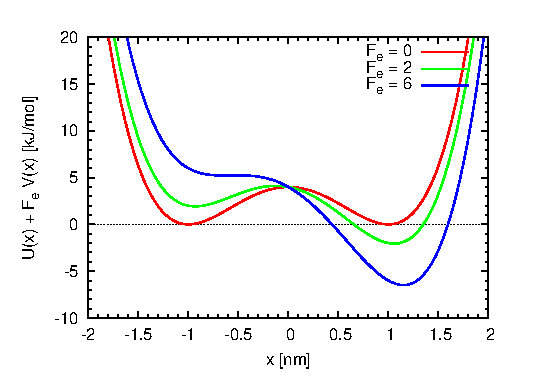
\includegraphics[width=8cm]{./fig.md/fig-pot.eps}
  \caption{The original dihedral potential and the dihedral potential
    with control.}
  \label{fig:tmp2}
\end{figure}


We considered $\lambda = 1.0$, 0.5, 0.2 and 0.1~ps and shown the
results in Fig.~\ref{fig:tmp2}, Tab.~\ref{tab:tmp1} and~\ref{tab:tmp2}.
From each of the 5000 equilibrium conformations, 4 trajectories with
different randoms seeds are simulated for each $\lambda$, so we
generate 20000 trajectories for each case.  The control $u(r, \omega)$ is
calculated by simulations of butane in vacumm, in which all other
parameters are the same as the aforementioned descriptions, except
that the waters are removed. We do it this way because the vacumm
simulation is much cheaper than the in-water simulation, and
practically, the control calculated in the corresponding vacumm
systems perform well enough in the in-water systems, because we find
that no further iteration is need to refine the control. Furthermore,
in the vacumm system, the probability $\mathcal{P}(\tau\leq\lambda) =
2.19\times10^{-2}$, $9.32\times 10^{-3}$, $1.35\times 10^{-3}$ and
$5.76\times 10^{-5}$ for $\lambda = 1.0$, 0.5, 0.2 and 0.1~ps,
respectively. These values does not significantly differ from the
dissolved system (see the second column of Tab.~\ref{tab:tmp1}).
Noticing the butane is symmetric with respect to transitional and
rotational movement, the above observation therefore indicates that
the transitional, rotational DOFs and the water structure does not
play a dominant role in the conformational change of butane, and the
definition of control only as a function as the dihedral angle, and
the computation of control in the vacumm system are reasonable
choices.  

\begin{table}[t]
  \centering
  \caption{
    Butane dissolved in water. The variance reduced estimate of the probability
    $\mathcal{P} (\tau \leq \lambda)$ by applying control on the dihedral angle.
    See the text for more details of the definition of the control.
    Column ``Error'' denotes the standard deviation of
    estimating the probablity $\mathcal{P} (\tau \leq \lambda)$.
    Column ``Var'' denotes the reduced variation of the esimate.
    ``Accel.''(acceleration) is the ratio between
    the reduced variance and the brute force variance (see Tab.~\ref{tab:tmp2}),
    which is the actual speed-up of the simulation.
    ``Traj. Usage'' dentoes percentage of trajectoies that changes
    to the trans conformation within time interval $[0,\lambda]$.
  }
  \label{tab:tmp1}
  \begin{tabular*}{0.9\textwidth}{@{\extracolsep{\fill}}lcccrr}
    \hline\hline
    $\lambda$ [ps] & $\mathcal{P} (\tau \leq \lambda)$ & Error & Var & Accel. & Traj. Usage \\\hline
    0.1 & $4.34\times 10^{-5}$ & $1.16\times 10^{-5}$ & $2.31\times10^{-6}$ &18.8 & 0.7\%\\
    0.2 & $9.03\times 10^{-4}$ & $0.77\times 10^{-4}$ & $1.19\times10^{-4}$ & 7.6 &10.0\%\\
    0.5 & $6.96\times 10^{-3}$ & $0.34\times 10^{-3}$ & $2.21\times10^{-3}$ & 3.1 &11.9\%\\
    1.0 & $1.68\times 10^{-2}$ & $0.06\times 10^{-2}$ & $6.30\times10^{-3}$ & 2.7 &13.4\%\\
    \hline\hline
  \end{tabular*}
  \caption{
    Butane dissolved in water, brute force simulations
    without any variance reduction. The meaning of the columns are the same
    as Tab.~\ref{tab:tmp1}.}\label{tab:tmp2}
  \begin{tabular*}{0.9\textwidth}{@{\extracolsep{\fill}}lcccrr}
    \hline\hline
    $\lambda$ [ps] & $\mathcal{P} (\tau \leq \lambda)$ & Error & Var & Accel. & Traj. Usage \\\hline
    0.2 & $7.46\times 10^{-4}$ & $2.36\times 10^{-4}$ & $7.46\times10^{-4}$ & 1.0 & 0.1\%\\
    0.5 & $6.94\times 10^{-3}$ & $0.72\times 10^{-3}$ & $6.89\times10^{-3}$ & 1.0 & 0.7\%\\
    1.0 & $1.61\times 10^{-2}$ & $0.11\times 10^{-2}$ & $1.59\times10^{-2}$ & 1.0 & 1.6\%\\
    \hline\hline
  \end{tabular*}
\end{table}

The Fig.~\ref{fig:tmp1} plots the effective dihedral angle energy,
which is the original dihedral energy $V_\phi(\phi)$ plus the control
$V_{\textrm{ctrl}}(\phi)$. We only show the effective energy in the
range $[40^\circ, 150^\circ]$, because the initial
conformations start in range $[40^\circ, 80^\circ]$, and the
trajectoies are stopped when they reach $\phi = 150^\circ$. For an easy
comparison, all effective energies are switched by a constant, so that
they are of vanishing value at $\phi = 150^\circ$. It clear that for
smaller $\lambda$ value, the control applied is stronger. Different
from the one-dimensional case, where the barrier is lowered, in this
case, only the potential well around $\phi = 60^\circ$ is fill, and
the barrier around $\phi = 120^\circ$ is almost kept the same.  The
resultant probability $\mathcal{P} (\tau \leq \lambda)$ calculated by the
variance reduced simulation is summarized in Tab.~\ref{tab:tmp1},
which is consistent with Tab.~\ref{tab:tmp2} that presents the
brute force results. Since the variance is redueced, the error of the
statistical esitmate is more precise in the variance reduced case. The
reduced variance is shown in the fourth column of Tab.~\ref{tab:tmp1},
which is much smaller than the brute force case (the fourth column of
Tab.~\ref{tab:tmp2}). The fifth column presents the acceleration ratio
with respect to the brute force simulation or the benefit from the
variance reduction, which is exactly the ratio between the brute force
variance and the reduced variance. The column of trajectory usage
presents the percentage of the trajectories that changes to the trans
conformation within time interval $[0, \lambda]$. It is increased by
the control with respect to the brute force result.




\section{Discussions}
\label{sec-discuss}

As a continuation of the work \cite{zlph2013, zhws13}, we study the cross-entropy
method in the setting of diffusion process and their application in the
importance sampling and optimal control.
In those previous work, some assumptions have been made on the dynamical systems and
on the type of quantities to estimate \cite{zhws13}. For example, 
in order to perform the asymptotic analysis, we assumed there are explicit parameters in dynamical systems and the dynamics
is in certain limit regime. In the case of multiple time-scale systems, we
also assumed that explicit slow/fast variables are known. In sampling problem \cite{zhws13}, we assumed 
the optimal change of measure is related to certain Hamilton-Jacobi-Bellman equation,
and therefore the type of quantity to estimate is restricted. With the
cross-entropy method, all these assumptions could be removed. General
diffusion processes can be investigated and importance sampling for more
meaningful quantity such as the probability $\mathcal{P}(\tau \le \lambda)$ can be considered.

On the other hand, some basis functions are needed in order to apply the
cross-entropy method. The choice of these basis functions are crucial in order
to obtain good approximation of the target measure and therefore effcient
importance sampling or ``good control force'' in the optimal control problem.
The successful choice is often based on our knowledge about the given dyanmical
system, such as its metastable states, or reactive cordinates. It is easy to
imagine that there is no way to obtain satisfactory results when the system
has a reactive coordinate but the basis functions are supported somewhere else.
The optimal control problem for dynamical systems having a reactive coordinate
will be further studied in the future work.

\section*{Acknowledgements}
The authors acknowledge financial support by the DFG Research Center MATHEON.
\FloatBarrier

\bibliographystyle{siam}
\bibliography{reference}
\end{document}
